\documentclass[11pt,compress,t,notes=noshow, xcolor=table]{beamer}
\usepackage[]{graphicx}\usepackage[]{color}
% maxwidth is the original width if it is less than linewidth
% otherwise use linewidth (to make sure the graphics do not exceed the margin)
\makeatletter
\def\maxwidth{ %
  \ifdim\Gin@nat@width>\linewidth
    \linewidth
  \else
    \Gin@nat@width
  \fi
}
\makeatother

\newcommand{\citebutton}[2]{%
\beamergotobutton{\href{#2}{#1}}%
}

\newcommand{\blu}[1]{\textcolor{blue}{#1}}
\newcommand{\org}[1]{\textcolor{orange}{#1}}
\newcommand{\ques}{\textbf{\textcolor{red}{Question:  }}}
\newcommand{\questionssofar}{\begin{frame}\frametitle{Any questions?}\end{frame}}

\newcommand\warning{%
 \makebox[1.4em][c]{%
 \makebox[0pt][c]{\raisebox{.1em}{\scriptsize!}}%
 \makebox[0pt][c]{\color{red}\normalsize$\bigtriangleup$}}}%

\definecolor{fgcolor}{rgb}{0.345, 0.345, 0.345}
\newcommand{\hlnum}[1]{\textcolor[rgb]{0.686,0.059,0.569}{#1}}%
\newcommand{\hlstr}[1]{\textcolor[rgb]{0.192,0.494,0.8}{#1}}%
\newcommand{\hlcom}[1]{\textcolor[rgb]{0.678,0.584,0.686}{\textit{#1}}}%
\newcommand{\hlopt}[1]{\textcolor[rgb]{0,0,0}{#1}}%
\newcommand{\hlstd}[1]{\textcolor[rgb]{0.345,0.345,0.345}{#1}}%
\newcommand{\hlkwa}[1]{\textcolor[rgb]{0.161,0.373,0.58}{\textbf{#1}}}%
\newcommand{\hlkwb}[1]{\textcolor[rgb]{0.69,0.353,0.396}{#1}}%
\newcommand{\hlkwc}[1]{\textcolor[rgb]{0.333,0.667,0.333}{#1}}%
\newcommand{\hlkwd}[1]{\textcolor[rgb]{0.737,0.353,0.396}{\textbf{#1}}}%
\let\hlipl\hlkwb

\usepackage{framed}
\makeatletter
\newenvironment{kframe}{%
 \def\at@end@of@kframe{}%
 \ifinner\ifhmode%
  \def\at@end@of@kframe{\end{minipage}}%
  \begin{minipage}{\columnwidth}%
 \fi\fi%
 \def\FrameCommand##1{\hskip\@totalleftmargin \hskip-\fboxsep
 \colorbox{shadecolor}{##1}\hskip-\fboxsep
     % There is no \\@totalrightmargin, so:
     \hskip-\linewidth \hskip-\@totalleftmargin \hskip\columnwidth}%
 \MakeFramed {\advance\hsize-\width
   \@totalleftmargin\z@ \linewidth\hsize
   \@setminipage}}%
 {\par\unskip\endMakeFramed%
 \at@end@of@kframe}
\makeatother

\definecolor{shadecolor}{rgb}{.97, .97, .97}
\definecolor{messagecolor}{rgb}{0, 0, 0}
\definecolor{warningcolor}{rgb}{1, 0, 1}
\definecolor{errorcolor}{rgb}{1, 0, 0}
\newenvironment{knitrout}{}{} % an empty environment to be redefined in TeX

\usepackage{alltt}
\newcommand{\SweaveOpts}[1]{}  % do not interfere with LaTeX
\newcommand{\SweaveInput}[1]{} % because they are not real TeX commands
\newcommand{\Sexpr}[1]{}       % will only be parsed by R
\newcommand{\xmark}{\ding{55}}%


\usepackage[english]{babel}
\usepackage[utf8]{inputenc}

\usepackage{dsfont}
\usepackage{verbatim}
\usepackage{amsmath}
\usepackage{amsfonts}
\usepackage{amssymb}
\usepackage{bm}
\usepackage{csquotes}
\usepackage{multirow}
\usepackage{longtable}
\usepackage{booktabs}
\usepackage{enumerate}
\usepackage[absolute,overlay]{textpos}
\usepackage{psfrag}
\usepackage{algorithm}
\usepackage{algpseudocode}
\usepackage{eqnarray}
\usepackage{arydshln}
\usepackage{tabularx}
\usepackage{placeins}
\usepackage{tikz}
\usepackage{setspace}
\usepackage{colortbl}
\usepackage{mathtools}
\usepackage{wrapfig}
\usepackage{bm}
\usepackage{amsmath}
\usepackage{pifont}

\usetikzlibrary{shapes.multipart,shapes,arrows,automata,positioning,calc,chains,trees, shadows}
\tikzset{
  %Define standard arrow tip
  >=stealth',
  %Define style for boxes
  punkt/.style={
    rectangle,
    rounded corners,
    draw=black, very thick,
    text width=6.5em,
    minimum height=2em,
    text centered},
  % Define arrow style
  pil/.style={
    ->,
    thick,
    shorten <=2pt,
    shorten >=2pt,}
}

\tikzstyle{vec}=[draw, rectangle, fill = white, minimum width=5mm, minimum height=1cm, inner sep = 2pt]

\usepackage{subfig}

% Defines macros and environments
\usepackage{../../style/lmu-lecture}


\let\code=\texttt
\let\proglang=\textsf

\setkeys{Gin}{width=0.9\textwidth}

\setbeamertemplate{frametitle}{\expandafter\uppercase\expandafter\insertframetitle}

\usepackage{bbm}
% basic latex stuff
\newcommand{\pkg}[1]{{\fontseries{b}\selectfont #1}} %fontstyle for R packages
\newcommand{\lz}{\vspace{0.5cm}} %vertical space
\newcommand{\dlz}{\vspace{1cm}} %double vertical space
\newcommand{\oneliner}[1] % Oneliner for important statements
{\begin{block}{}\begin{center}\begin{Large}#1\end{Large}\end{center}\end{block}}


%new environments
\newenvironment{vbframe}  %frame with breaks and verbatim
{
 \begin{frame}[containsverbatim,allowframebreaks]
}
{
\end{frame}
}

\newenvironment{vframe}  %frame with verbatim without breaks (to avoid numbering one slided frames)
{
 \begin{frame}[containsverbatim]
}
{
\end{frame}
}

\newenvironment{blocki}[1]   % itemize block
{
 \begin{block}{#1}\begin{itemize}
}
{
\end{itemize}\end{block}
}

\newenvironment{fragileframe}[2]{  %fragile frame with framebreaks
\begin{frame}[allowframebreaks, fragile, environment = fragileframe]
\frametitle{#1}
#2}
{\end{frame}}


\newcommand{\myframe}[2]{  %short for frame with framebreaks
\begin{frame}[allowframebreaks]
\frametitle{#1}
#2
\end{frame}}

\newcommand{\remark}[1]{
  \textbf{Remark:} #1
}


\newenvironment{deleteframe}
{
\begingroup
\usebackgroundtemplate{
\includegraphics[width=\paperwidth,height=\paperheight]{../style/color/red.png}}
 \begin{frame}
}
{
\end{frame}
\endgroup
}
\newenvironment{simplifyframe}
{
\begingroup
\usebackgroundtemplate{
\includegraphics[width=\paperwidth,height=\paperheight]{../style/color/yellow.png}}
 \begin{frame}
}
{
\end{frame}
\endgroup
}\newenvironment{draftframe}
{
\begingroup
\usebackgroundtemplate{
\includegraphics[width=\paperwidth,height=\paperheight]{../style/color/green.jpg}}
 \begin{frame}
}
{
\end{frame}
\endgroup
}
% https://tex.stackexchange.com/a/261480: textcolor that works in mathmode
\makeatletter
\renewcommand*{\@textcolor}[3]{%
  \protect\leavevmode
  \begingroup
    \color#1{#2}#3%
  \endgroup
}
\makeatother





\input{../../latex-math/basic-math.tex}
\input{../../latex-math/basic-ml.tex}

\newcommand{\titlefigure}{figure/sesamestreet.jpeg}
\newcommand{\learninggoals}{
\item Understand the improvements over BERT
\item Dynamic Masking}

\title{Using the Transformer}
% \author{}
\institute{\href{https://slds-lmu.github.io/lecture_dl4nlp/}{slds-lmu.github.io/lecture\_dl4nlp}}
\date{}

\begin{document}
\lecturechapter{RoBERTa (Liu et al., 2019)}
\lecture{Deep Learning for NLP}

% ------------------------------------------------------------------------------

\begin{frame}{Improvements in Pre-Training}

\vfill

	\textbf{Short summary:}

	\begin{itemize}
		\item Change of the \texttt{MASK}ing strategy  \\
					$\rightarrow$ BERT masks the sequences once before pre-training  \\
					$\rightarrow$ RoBERTa uses dynamic \texttt{MASK}ing  \\
					$\Rightarrow$ RoBERTa sees the same sequence \texttt{MASK}ed differently
		\item RoBERTa does not use the additional NSP objective during pre-training
		\item Authors claim that BERT is seriously "undertrained"
			\begin{itemize}
				\item 160 GB of pre-training resources instead of 13 GB
				\item Pre-training is performed with larger batch sizes (8k)
			\end{itemize}
	\end{itemize}
	
\vfill

\end{frame}

% ------------------------------------------------------------------------------

\begin{frame}{Dynamic vs. Static Masking}

\vfill

	\textbf{Static Masking (BERT):}

	\begin{itemize}
		\item Apply \texttt{MASK}ing procedure to pre-training corpus once
		\item (additional for BERT: Modify the corpus for NSP)
		\item Train for approximately 40 epochs
	\end{itemize}

\vspace{.3cm}

	\textbf{Dynamic Masking (RoBERTa):}

	\begin{itemize}
		\item Duplicate the training corpus \textit{ten} times
		\item Apply \texttt{MASK}ing procedure to each duplicate of the pre-training corpus
		\item Train for 40 epochs
		\item Model sees each training instance in ten different "versions"\\
					(each version four times) during pre-training
	\end{itemize}
	
\vfill

\end{frame}

% ------------------------------------------------------------------------------

\begin{frame}{Dynamic vs. Static Masking}

\vfill

\begin{figure}
\centering
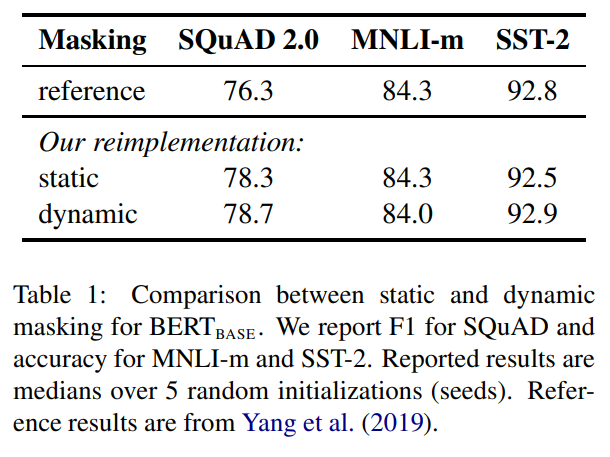
\includegraphics[width = 8cm]{figure/roberta-dynamic.png}\\ 
\footnotesize{Source:} \href{https://arxiv.org/pdf/1907.11692.pdf}{\footnotesize Liu et al. (2019)}
\end{figure}

\vfill

\end{frame}

% ------------------------------------------------------------------------------

\begin{frame}{No NSP}

\vfill

	\begin{itemize}
		\item Described as important part of the pre-training process in BERT
		\item Liu et al. report that it hurts performance
		\item[$\to$] Especially for QNLI, MNLI, and SQuAD 1.1
		\item Conduct experiments in multiple settings: 
			\begin{itemize}
				\item SEGMENT-PAIR+NSP
				\item SENTENCE-PAIR+NSP
				\item FULL-SENTENCES
				\item DOC-SENTENCES
			\end{itemize}
	\end{itemize}
	
\vfill

\end{frame}

% ------------------------------------------------------------------------------
\begin{frame}{RoBERTa \href{https://arxiv.org/pdf/1907.11692.pdf}{\beamergotobutton{Liu et al., 2019}}}

\vfill

\begin{figure}
\centering
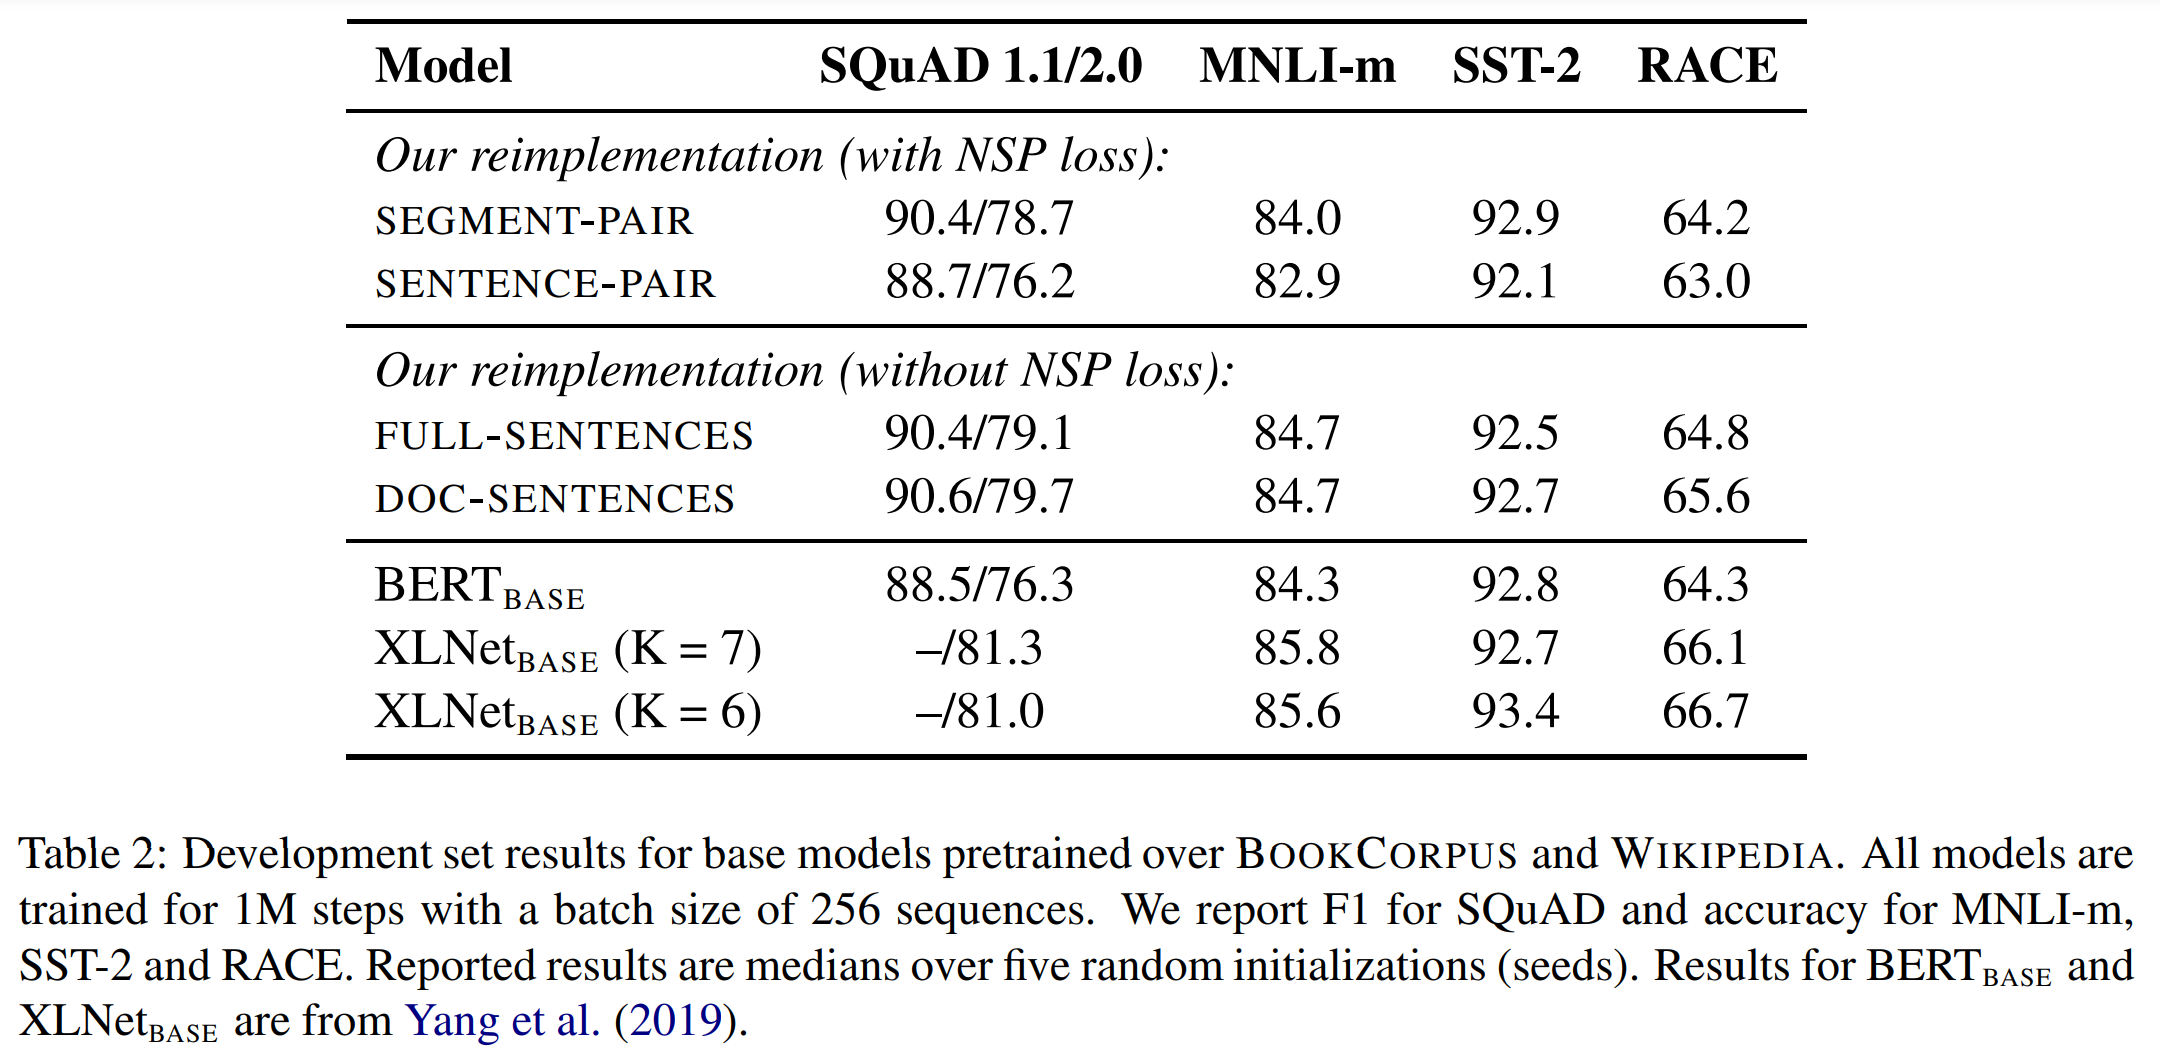
\includegraphics[width = 11cm]{figure/roberta-nsp.png}\\ 
\footnotesize{Source:} \href{https://arxiv.org/pdf/1907.11692.pdf}{\footnotesize Liu et al. (2019)}
\end{figure}
\footnotesize
\textit{Note:} XLNet: see next Chapter.

\vfill

\end{frame}

% ------------------------------------------------------------------------------

\begin{frame}{Changes in pre-training}

\vfill

\begin{figure}
\centering
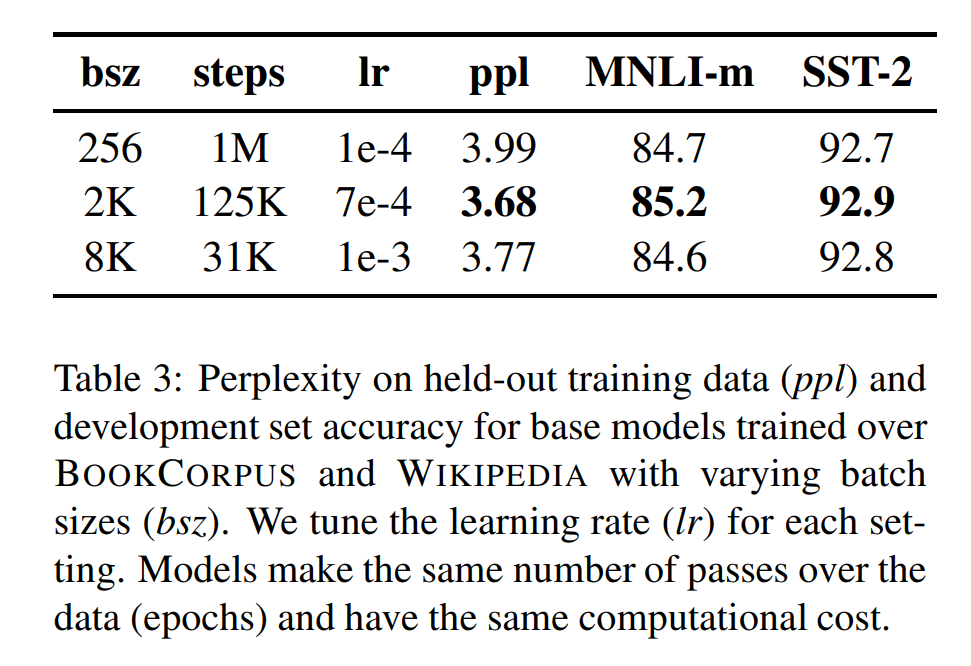
\includegraphics[width = 8cm]{figure/roberta-undertrained.png}\\ 
\footnotesize{Source:} \href{https://arxiv.org/pdf/1907.11692.pdf}{\footnotesize Liu et al. (2019)}
\end{figure}

\vfill

\end{frame}

% ------------------------------------------------------------------------------

\begin{frame}{Changes in pre-training}

\vfill

\begin{figure}
\centering
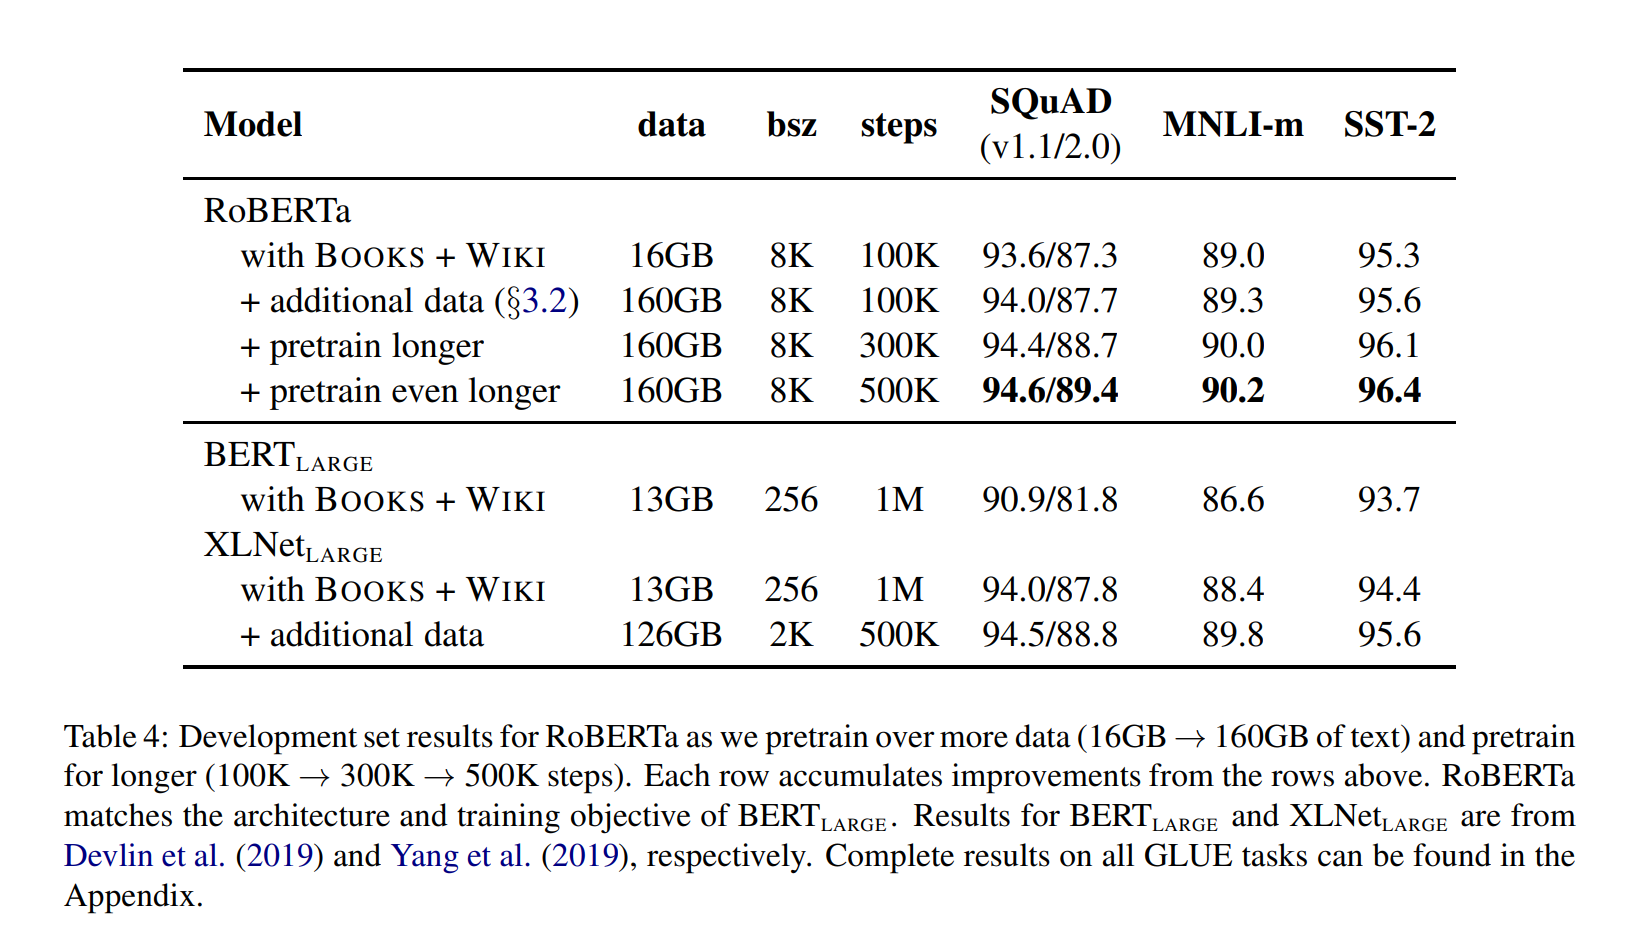
\includegraphics[width = 11cm]{figure/roberta-undertrained2.png}\\ 
\footnotesize{Source:} \href{https://arxiv.org/pdf/1907.11692.pdf}{\footnotesize Liu et al. (2019)}
\end{figure}
\footnotesize
\textit{Note:} XLNet: see next Chapter.

\vfill

\end{frame}

% ------------------------------------------------------------------------------
\begin{frame}{RoBERTa \href{https://arxiv.org/pdf/1907.11692.pdf}{\beamergotobutton{Liu et al., 2019}}}

\textbf{Architectural differences:}

\begin{itemize}
\item Architecture (layers, heads, embedding size) identical to BERT
\item 50k token BPE vocabulary instead of 30k
\item Model size differs (due to the larger embedding matrix)\\
			$\Rightarrow$ $\sim$ 125M (360M) for the BASE (LARGE) variant 
\end{itemize}

\textbf{Performance differences:}

\begin{figure}
\centering
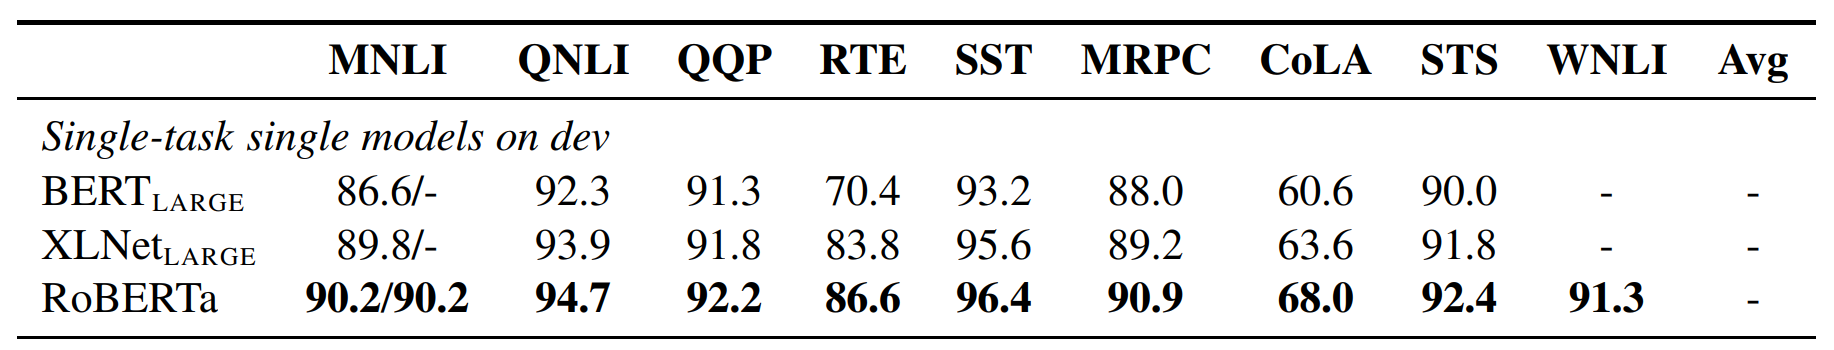
\includegraphics[width = 11cm]{figure/roberta-sota.png}\\ 
\footnotesize{Source:} \href{https://arxiv.org/pdf/1907.11692.pdf}{\footnotesize Liu et al. (2019)}
\end{figure}
\footnotesize
\textit{Note:} Liu et al. (2019) report the accuracy for QQP while Devlin et al. (2018) report the F1 score (cf. results displayed in chapter 6.2.3); XLNet: see next Chapter.
\end{frame}
% ------------------------------------------------------------------------------

\endlecture
\end{document}
